\documentclass[10pt,a4paper]{article}
\usepackage[utf8]{inputenc}
\usepackage[T1]{fontenc}
\usepackage[colorlinks=true]{hyperref}
\usepackage{amsmath}
\usepackage{amssymb}
\usepackage{graphicx}
\usepackage{dirtree}
\usepackage[left=2.00cm, right=2.00cm, top=2.00cm, bottom=2.00cm]{geometry}

%%%%%%%%%%%%%%%%%%%% default %%%%%%%%%%%%%%%
%\makeatletter
%\def\@maketitle{%
%	\newpage
%	\null
%	\vskip 2em%
%	\begin{center}%
%		\let \footnote \thanks
%		{\LARGE \@title \par}%
%		\vskip 1.5em%
%		{\large \@author\par}%
%		\vskip 1em%
%		{\large
%			\lineskip .5em%
%			\begin{tabular}[t]{c}%
%				\@date
%		\end{tabular}}%
%	\end{center}%
%	\par
%	\vskip 1.5em}
%\makeatother
%%%%%%%%%%%%%%%%%%%%%%%%%%%%

%%%%%%%%%%%%%%%%%%%% change title %%%%%%%%%%%%%%%
\makeatletter
\def\@maketitle{%
		\null
		\vskip 2em%
		\begin{center}%
				\let \footnote \thanks
				{\LARGE \@title \par}%
				\vskip 3em%
				{\LARGE \@author\par}%
				\vskip 30em%
				{\large
						\lineskip .5em%
						\begin{tabular}[t]{c}%
								\@date
						\end{tabular}}%
			\end{center}%
		\par
		\vskip 1.5em}
\makeatother
%%%%%%%%%%%%%%%%%%%%%%%%%%%%

%%%%%%%%%%%%%%% Another Way %%%%%%%%%%%%%%
%\begin{titlepage}
%	\vspace*{\stretch{1}}
%	\begin{center}
%		{\huge\bfseries Thesis \\[1ex] 
%			title}                  \\[6.5ex]
%		{\large\bfseries Author name}           \\
%		Thesis  submitted to                    \\[5pt]
%		\textit{University name}                \\[2cm]
%		in partial fulfilment for the award of the degree of \\[2cm]
%		\textsc{\Large Doctor of Philosophy}    \\[2ex]
%		\textsc{\large Mathematics}             \\[12ex]
%		\vfill
%		Department of Mathematics               \\
%		Address                                 \\
%		\vfill
%		\today
%	\end{center}
%	\vspace{\stretch{2}}
%\end{titlepage}
%%%%%%%%%%%%%%%%%%%%%%%%%%%%%%%%%%%%%%

\title{Computational Fluid Dynamics Coursework\\
\qquad\qquad\qquad\qquad\qquad{Numerical Simulation of Shallow Water Wave}
\author{Xu Duan}
%\date{}
\newcommand{\td}{\mbox{d}}
\newcommand{\upcite}[1]{\textsuperscript{\zihao{5}\cite{#1}}}

\begin{document}
	\thispagestyle{empty}
	\newpage
	\begin{figure}
		\center{\includegraphics[width=5cm]{fig1.png}}
	\end{figure}
	\maketitle
	\newpage
	\pagenumbering{Roman}
	\tableofcontents
	\newpage
	\pagenumbering{arabic}
	\setcounter{page}{1}
\section{Problem Description}
Coastal tides are typical shallow water waves, usually with a small ratio of depth to wavelength, hence they are also called long waves. We hope to numerically simulate the evolution and deformation of distant harmonic tidal waves as they propagate towards the shore, as the water depth gradually decreases. For this purpose, a rectangular pool is designed to calculate the operating conditions, with a length of 800 meters. The west side of the pool is 400 meters of horizontal seabed with a depth of 10 meters, and the east side of the pool is 400 meters of inclined seabed with a linear decrease in depth from 10 to 0. As shown in the following figure
\begin{figure}[h]
	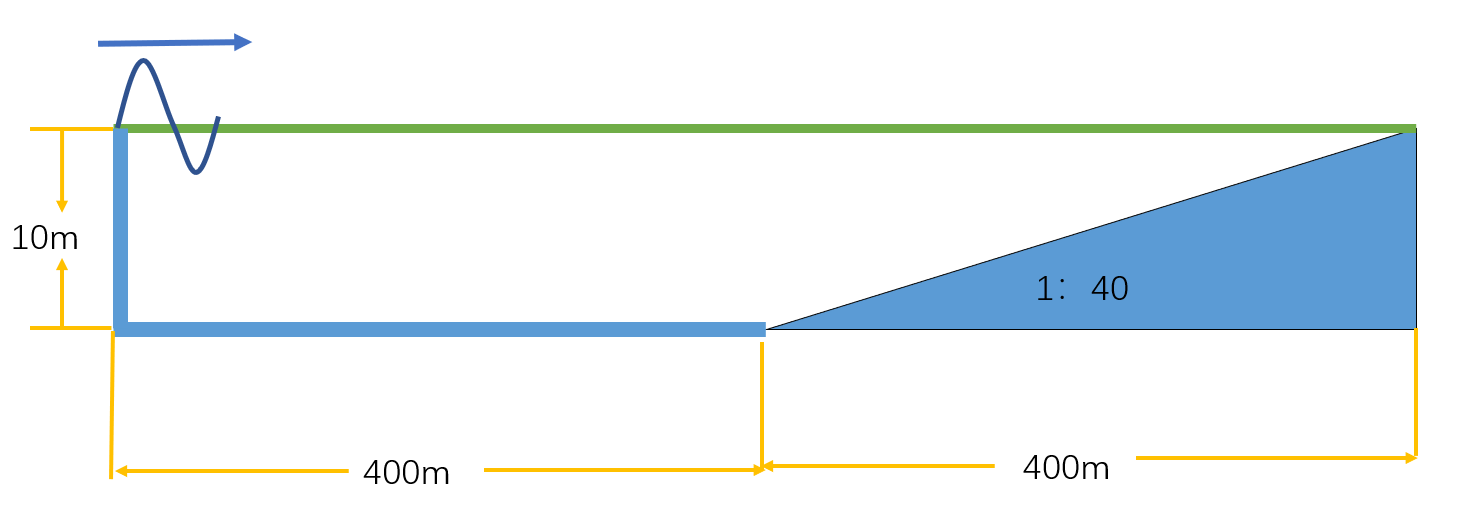
\includegraphics[width=\textwidth]{sideTank.png}
	\caption{Side view}
\end{figure}
\begin{figure}[h]
	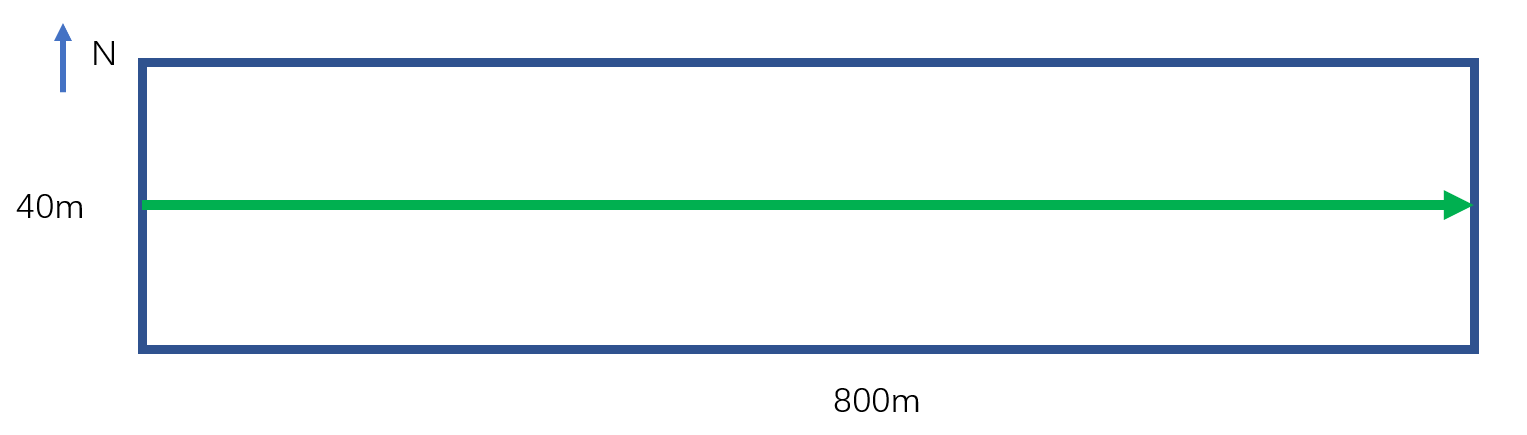
\includegraphics[width=\textwidth]{topTank.png}
	\caption{Vertical view}
\end{figure}

The regular wave enters from the west side, amplitude is $0.5\mbox{m}$, period is $8\mbox{s}$. Explore the patterns of deformation of regular waves on this terrain.
\newpage
\section{Basic Theory}
\subsection{Governing Equations}
	Define wavefront shape as a function $z = H(x, y, t)$, Underwater terrain function $z = -D(x, y)$, as shown in the following figure\upcite{1}
\begin{figure}[h]
	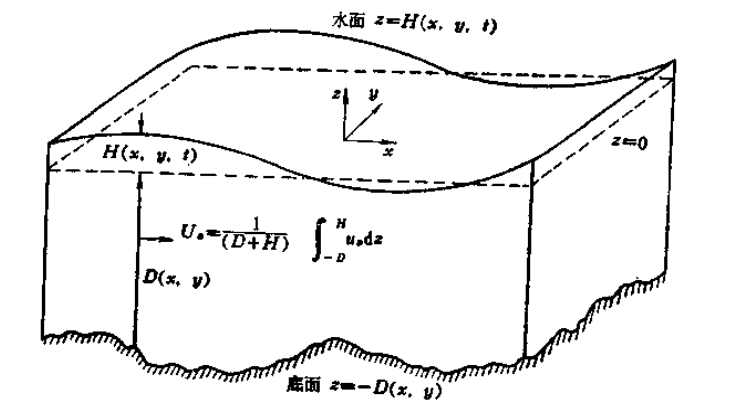
\includegraphics[width=\textwidth]{coordinates.png}
	\caption{Definition of Coordinate System}
\end{figure}

Introduce the average velocity in shallow water waves
\begin{equation}
	\begin{aligned}
		U &= \frac{1}{D+H}\int_{-D}^{H}u \td z\\
		V &= \frac{1}{D+H}\int_{-D}^{H}v \td z
	\end{aligned}
\end{equation}

Then, by the principle of conservation of mass (Continuity equation)
\begin{equation*}
	\frac{\partial w}{\partial z}  = -\frac{\partial u}{\partial x} - \frac{\partial v}{\partial y}
\end{equation*}
integrate from $-D$ to $-H$ gives
\begin{equation}\label{mc}
	w|_H - w|_{-D}  = -\int_{-D}^{H}\frac{\partial u}{\partial x} + \frac{\partial v}{\partial y} \td z
\end{equation}
By free surface boundary conditions
\begin{equation}\label{bcf}
	w|_H  = u\frac{\partial H}{\partial x} + v\frac{\partial H}{\partial y} + \frac{\partial H}{\partial t}
\end{equation}
Due to underwater conditions
\begin{equation}\label{bcb}
	w|_{-D}  = -u\frac{\partial H}{\partial x} - v\frac{\partial H}{\partial y}
\end{equation}
from (\ref{mc})(\ref{bcf})(\ref{bcb}) and the following relation
\begin{equation*}
	\begin{aligned}
		\frac{\partial}{\partial x}\int_{-D}^{H}u\td z &= \int_{-D}^{H}\frac{\partial u}{\partial x}\td z + u|_H\frac{\partial H}{\partial x} + u|_{-D}\frac{\partial D}{\partial x}\\
		\frac{\partial}{\partial y}\int_{-D}^{H}v\td z &= \int_{-D}^{H}\frac{\partial v}{\partial y}\td z + v|_H\frac{\partial H}{\partial y} + v|_{-D}\frac{\partial D}{\partial y}
	\end{aligned}
\end{equation*}

Can be obtained
\begin{equation}
	\frac{\partial H}{\partial t} + \frac{\partial}{\partial x}\int_{-D}^{H}u\td z + \frac{\partial}{\partial y}\int_{-D}^{H}v\td z = 0
\end{equation}
namely
\begin{equation}\label{mass}
	\frac{\partial H}{\partial t} + \frac{\partial (D+H)U}{\partial x} + \frac{\partial (D+H)V}{\partial y} = 0
\end{equation}
From the conservation of momentum (ignoring viscosity), we can obtain
\begin{equation}
	\begin{aligned}
		\frac{\partial U}{\partial t} + U\frac{\partial U}{\partial x} + V\frac{\partial U}{\partial y} + W\frac{\partial U}{\partial z} = - \frac{1}{\rho}\frac{\partial p}{x} + F_x\\
		\frac{\partial V}{\partial t} + U\frac{\partial V}{\partial x} + V\frac{\partial V}{\partial y} + W\frac{\partial V}{\partial z} = - \frac{1}{\rho}\frac{\partial p}{y} + F_y\\
		\frac{\partial W}{\partial t} + U\frac{\partial W}{\partial x} + V\frac{\partial W}{\partial y} + W\frac{\partial W}{\partial z} = - \frac{1}{\rho}\frac{\partial p}{z} - g
	\end{aligned}
\end{equation}
In shallow water, velocity in $z$direction, $W$ can be ignored. so, from the momentum conservation in $z$ direction, it is obtained that
\begin{equation*}
	p(z) = \rho g (H - z)
\end{equation*}
Then
\begin{equation*}
	\begin{aligned}
		\frac{1}{\rho}\frac{\partial p}{\partial x} &= g \frac{\partial H}{\partial x}\\
		\frac{1}{\rho}\frac{\partial p}{\partial y} &= g \frac{\partial H}{\partial y}
	\end{aligned}
\end{equation*}
substituting into the momentum equation in $x $and $y $directions, it is obtained that
\begin{equation}
	\begin{aligned}
		\frac{\partial U}{\partial t} + U\frac{\partial U}{\partial x} + V\frac{\partial U}{\partial y} + g\frac{\partial H}{\partial x} = F_x\\
		\frac{\partial V}{\partial t} + U\frac{\partial V}{\partial x} + V\frac{\partial V}{\partial y} + g\frac{\partial H}{\partial y} = F_y
	\end{aligned}
\end{equation}
The external force term can be expressed as
\begin{equation}
	\begin{aligned}
		F_x &= FV + F^{(x)} + \tau_x\\
		F_y &= -FU + F^{(y)} + \tau_y
	\end{aligned}
\end{equation}
The first term on the right side of the equation is the Coriolis force.
\begin{equation}
	F = 2 \Omega \sin\phi
\end{equation}
where $\Omega$ is Earth's rotational angular velocity. $\Omega = 1.46\times10^{-4}s^{-1}$. $\phi$ is latitude, which is taken to be 31°. So, $$F = 1.5\times10^{-4}s^{-1}$$.

The second term on the right-hand side of the equation is wind force. This example does not take into account wind power.

The third term on the right side of the equation is the seabed friction force. According to Drkonkers\upcite{2}
\begin{equation}
	\tau_b = \rho g C^{-2}\boldsymbol{U}|\boldsymbol{U}|
\end{equation}
where $C$ is Chezy constant, which is taken to be $C = 25$.
Based on the above equations, the momentum equation is transformed into
\begin{equation}\label{momentum}
	\begin{aligned}
		&\frac{\partial U}{\partial t} + U\frac{\partial U}{\partial x} + V\frac{\partial U}{\partial y} + g\frac{\partial H}{\partial x} = FV - g\frac{U(U^2 + V^2)^{\frac{1}{2}}}{C^2(D+H)}\\
		&\frac{\partial V}{\partial t} + U\frac{\partial V}{\partial x} + V\frac{\partial V}{\partial y} + g\frac{\partial H}{\partial y} = -FU - g\frac{V(U^2 + V^2)^{\frac{1}{2}}}{C^2(D+H)}
	\end{aligned}
\end{equation}

The governing equation for shallow water waves is summarized as follows:
\begin{equation}\label{control}
	\begin{aligned}
		&\frac{\partial H}{\partial t} + \frac{\partial (D+H)U}{\partial x} + \frac{\partial (D+H)V}{\partial y} = 0\\
		&\frac{\partial U}{\partial t} + U\frac{\partial U}{\partial x} + V\frac{\partial U}{\partial y} + g\frac{\partial H}{\partial x} = FV - g\frac{U(U^2 + V^2)^{\frac{1}{2}}}{C^2(D+H)}\\
		&\frac{\partial V}{\partial t} + U\frac{\partial V}{\partial x} + V\frac{\partial V}{\partial y} + g\frac{\partial H}{\partial y} = -FU - g\frac{V(U^2 + V^2)^{\frac{1}{2}}}{C^2(D+H)}
	\end{aligned}
\end{equation}

\subsection{Boundary Conditions}\label{bc}
To solve this system of partial differential equations, boundary conditions need to be given
\begin{equation}
	\begin{aligned}
		H|_\Gamma = H_\Gamma (t)\\
		U|_\Gamma = U_\Gamma (t)\\
		V|_\Gamma = V_\Gamma (t)\\
	\end{aligned}
\end{equation}
For this example, the boundary conditions on the north, south, and east sides are continuous conditions, that is, the grid at the boundary is obtained by linearly extrapolating the values at the grid points within the boundary.

The western boundary condition is the input harmonic wave, The velocity in $x$ direction can be expressed as
\begin{equation}
	u = A\omega\frac{\cosh k(z+D)}{\sinh kD} \cos\omega t
\end{equation}
when $D\to0$, $\cosh k(z+D) \to 1$, $\sinh kD \to kD$. The western boundary condition is
\begin{equation}
	\begin{aligned}
		H &= A\cos\omega t\\
		U &= \frac{A\omega}{kD}\cos\omega t = A\sqrt{\frac{g}{D}}\cos\omega t\\
		V &= 0
	\end{aligned}
\end{equation}
\subsection{Initial Condition}
Initial Condition is set to be zero, namely
\begin{equation}
	\begin{aligned}
		H(x, y, t)|_{t= 0} = 0\\
		U(x, y, t)|_{t= 0} = 0\\
		V(x, y, t)|_{t= 0} = 0
	\end{aligned}
\end{equation}
\newpage
\section{Numerical Schemes}
\subsection{Introduction to Numerical Schemes}\label{spacedis}
The spatial discretization method adopts the upwind format \upcite{3} while The time is stepped in Euler format.

For mass conservation equation(\ref{mass}), the following discretized form is obtained
\begin{equation}
	H_{i, j}^{n+1} = H_{i, j}^n - \Delta t\left[\frac{U_{i+1, j}^n}{\Delta x}(TD1) - \frac{U_{i, j}^n}{\Delta x}(TD2) + \frac{V_{i, j+1}^n}{\Delta y}(TV1) - \frac{V_{i, j}^n}{\Delta y}(TV2)\right]
\end{equation}
where
\begin{equation}
	\begin{aligned}
		TD1 &= D_{i+1, j} + H_{i+1, j}^n\qquad (U_{i+1, j}^n < 0)\\
		\mbox{or} \qquad TD1 &= D_{i, j} + H_{i, j}^n\qquad (U_{i+1, j}^n > 0)\\
		TD2 &= D_{i, j} + H_{i, j}^n\qquad (U_{i, j}^n < 0) \\
		\mbox{or} \qquad TD2 &= D_{i-1, j} + H_{i-1, j}^n\qquad (U_{i, j}^n > 0) \\
		TV1 &= D_{i, j+1} + H_{i, j+1}^n\qquad (V_{i, j+1}^n < 0)\\
		\mbox{or} \qquad TV1 &= D_{i, j} + H_{i, j}^n\qquad (V_{i, j+1}^n > 0)\\
		TV2 &= D_{i, j} + H_{i, j}^n\qquad (V_{i, j}^n < 0)\\
		\mbox{or} \qquad TV2 &= D_{i, j-1} + H_{i, j-1}^n\qquad (V_{i, j}^n > 0)
	\end{aligned}
\end{equation}

For momentum conservation equation
\begin{equation}
	U_{i, j}^{n+1} = U_{i, j}^n - \Delta t\left[\frac{U_{i, j}^n}{\Delta x}(TU1) + \frac{TV}{\Delta y}(TU2)\right] + g\frac{\Delta t}{\Delta x}THU - \Delta t\left(-FV_{i, j}^n + S_{i, j}^{An}\right)
\end{equation}
where
\begin{equation}
	\begin{aligned}
		TU1 &= U_{i+1, j}^n - U_{i, j}^n\qquad (U_{i, j}^n < 0)\\
		\mbox{or} \qquad TU1 &= U_{i, j}^n - U_{i-1, j}^n\qquad (U_{i, j}^n > 0)\\
		TV &= \frac{1}{4}\left(V_{i-1, j} + V_{i+1, j} + V_{i, j-1} + V_{i, j+1}\right)\\
		TU2 &= U_{i, j+1}^n - U_{i, j}^n\qquad (TV < 0) \\
		\mbox{or} \qquad TU2 &= U_{i, j}^n - U_{i, j-1}^n\qquad (TV > 0) \\
		THU &= H_{i, j}^n - H_{i-1, j}^n \\
		S_{i, j}^{An} &= g\frac{U_{i, j}^n\left[(U_{i, j}^n)^2 + (V_{i, j}^n)^2\right]^{\frac{1}{2}}}{C^2(D_{i, j}+H_{i, j}^n)} \\
	\end{aligned}
\end{equation}
and
\begin{equation}
	V_{i, j}^{n+1} = V_{i, j}^n - \Delta t\left[\frac{TU}{\Delta x}(TV1) + \frac{V_{i, j}^n}{\Delta y}(TV2)\right] + g\frac{\Delta t}{\Delta y}THV - \Delta t\left(FU_{i, j}^n + S_{i, j}^{Bn}\right)
\end{equation}
where
\begin{equation}
	\begin{aligned}
		TU &= \frac{1}{4}\left(U_{i-1, j} + U_{i+1, j} + U_{i, j-1} + U_{i, j+1}\right)\\
		TV1 &= V_{i+1, j}^n - V_{i, j}^n\qquad (TU < 0)\\
		\mbox{or} \qquad TV1 &= V_{i, j}^n - V_{i-1, j}^n\qquad (TU > 0)\\
		TV2 &= V_{i, j+1}^n - V_{i, j}^n\qquad (V_{i, j} < 0) \\
		\mbox{or} \qquad TV2 &= V_{i, j}^n - V_{i, j-1}^n\qquad (V_{i, j} > 0) \\
		THV &= H_{i, j}^n - H_{i, j-1}^n \\
		S_{i, j}^{Bn} &= g\frac{V_{i, j}^n\left[(U_{i, j}^n)^2 + (V_{i, j}^n)^2\right]^{\frac{1}{2}}}{C^2(D_{i, j}+H_{i, j}^n)} \\
	\end{aligned}
\end{equation}

Due to the use of a first-order upwind format in the space, numerical values of the left and right nodes are required at the boundary, so a extra grid is added in the east, west, north, and south directions as boundaries.

Higher order time stepping schemes can also be used, such as Runge Kutta third-order integration and Runge Kutta fourth-order integration. Taking the rise of wave surface as an example, the following is a brief introduction:
\begin{equation}
	\Delta H = F(H^n)
\end{equation}
Euler method can be expressed as
\begin{equation}
	\begin{aligned}
		\Delta H_1 &= F(H^n)\\
		H^{n+1} &= H^n + \Delta H_1
	\end{aligned}
\end{equation}
The expression of Runge Kutta third-order integral is
\begin{equation}
	\begin{aligned}
		\Delta H_1 &= F(H^n)\\
		\Delta H_2 &= F(H^n + \Delta H_1)\\
		\Delta H_3 &= F(H^n + \frac{1}{4}\Delta H_1 + \frac{1}{4}\Delta H_2)\\
		H^{n+1} &= H^n + \frac{1}{6}\Delta H_1 + \frac{1}{6}\Delta H_2 + \frac{2}{3}\Delta H_3
	\end{aligned}
\end{equation}
The fourth order integral of Runge Kutta is expressed as
\begin{equation}
	\begin{aligned}
		\Delta H_1 &= F(H^n)\\
		\Delta H_2 &= F(H^n + \frac{1}{2}\Delta H_1)\\
		\Delta H_3 &= F(H^n + \frac{1}{2}\Delta H_2)\\
		\Delta H_4 &= F(H^n + \Delta H_3)\\
		H^{n+1} &= H^n + \frac{1}{6}\Delta H_1 + \frac{1}{3}\Delta H_2 + \frac{1}{3}\Delta H_3 + \frac{1}{6}\Delta H_4
	\end{aligned}
\end{equation}
\subsection{Error and Convergence Analysis}
For the upwind scheme and Euler method, the error of the difference scheme can be obtained as follows: $O(\Delta x) + O(\Delta t)$. If the time step format is changed to Runge Kutta third-order integration, the error is $O(\Delta x) + O(\Delta t^3)$. Similarly, for the Runge Kutta fourth-order integral, the error term is $O(\Delta x) + O(\Delta t^4)$.

According to the CFL condition, a necessary condition for calculating convergence is that the dependency region of the difference scheme includes the dependency region of the differential equation. Obviously, the upwind scheme is conditionally convergent for the following equation
\begin{equation}
	\frac{\partial f}{\partial t} + a \frac{\partial f}{\partial x} = 0
\end{equation}
The CFL condition is
\begin{equation}
	a\Delta t / \Delta x \le 1
\end{equation}
Therefore, if we only consider the conservation of mass equation(\ref{mass}) according \cite{4}, we choose
\begin{equation}
	a = \frac{1}{C}\max\left(\max|U_{i, j}| + \sqrt{g(D_{i, j} + H_{i, j})}, \max|V_{i, j}| + \sqrt{g(D_{i, j} + H_{i, j})}\right)
\end{equation}
Then 
\begin{equation}\label{convergence}
	\Delta t \le C\min\left(\min\frac{\Delta x}{|u_{i, j}| + \sqrt{g(D_{i, j} + H_{i, j})}}, \min\frac{\Delta y}{|v_{i, j}| + \sqrt{g(D_{i, j} + H_{i, j})}}\right)
\end{equation}
Among them, C is the Courant constant, generally $C = 0.5$.
\subsection{Introduction to Computational Programs}
The calculation program is written in Fortran and is mainly divided into three parts: \ textit {main.f90, helper. f90}, and \ textit {timestep. f90}. The file structure diagram is shown below
\\
\\
\\
\\
\dirtree{%
	.1 /.
	.2 src/.
	.3 main.f90.
	.3 helper.f90.
	.4 get\_input.
	.4 get\_init\_depth.
	.4 init.
	.4 show\_progress.
	.4 write\_output.
	.3 timestep.f90.
	.4 diffcalc.
	.4 bc.
	.2 input.txt.
	.2 depth.txt.
	.2 output/.
	.3 depth.txt.
	.3 h\_xxxxx.out.
	.3 u\_xxxxx.out.
	.3 v\_xxxxx.out.
	.2 Makefile.
	.2 postProcess.py.
}

where \textit{main.f90} is main program, doing initialization through calling \textit{helper.f90} and \textit{timestep.f90}, and time-step through a loop.

\textit{helper.f90} contains auxiliary functions in calculation, where \textit{get\_input}get Grid size, number of grids, step time interval, total simulation time, output time interval, and parameters of input regular waves (including circle frequency and amplitude) through reading \textit{input.txt} in the same directory.

\textit{get\_init\_depth} obtains the water depth through reading \textit{depth.txt} in the same directory and use linear extrapolation to obtain the water depth at the boundary grid points.

\textit{init} impose initial condition, setting wave elevation and speed to be zero.

\textit{show\_progress} shows progress, print result to the screen every $10\%$.

\textit{write\_output}put all output files into \textit{output} folder, outputting wave height field and velocity field each time, according to output time interval read by \textit{get\_input},

\textit{timestep.f90} contains \textit{diffcalc} function implementing the spatial discretization and time stepping methods described in\ref{spacedis}. function \textit{bc} impose boundary condition on west boundary as described in \ref{bc}.

\textit{Makefile} is the control file for compilation.

\textit{postProcess.py} is post-processing visualization program written in Python.
\newpage
\section{Results and Analysis}
\subsection{Verification of input waves}
Set $\td x= 2 \mbox{m}$, $\td y = 4 \mbox{m}$, according to (\ref{convergence}). Approximate calculation of time step size equals
\begin{equation}
	\begin{aligned}
		\Delta t &\le C\min\left(\min\frac{\Delta x}{|u_{i, j}| + \sqrt{g(D_{i, j} + H_{i, j})}}, \min\frac{\Delta y}{|v_{i, j}| + \sqrt{g(D_{i, j} + H_{i, j})}}\right) \\ &\le C\min\frac{\Delta x}{|u_{i, j}| + \sqrt{g(D_{i, j} + H_{i, j})}}\\
		&\approx 0.5\frac{2}{0.5 + \sqrt{9.8\times10}}\\
		&\approx 0.096\mbox{s}
	\end{aligned}
\end{equation}
set $\Delta t=0.01\mbox{s}$ and $\Delta t=0.001\mbox{s}$. Using the Euler method, draw the wave height history of two different time intervals on the west side of the pool as follows

\begin{figure}[htbp]
	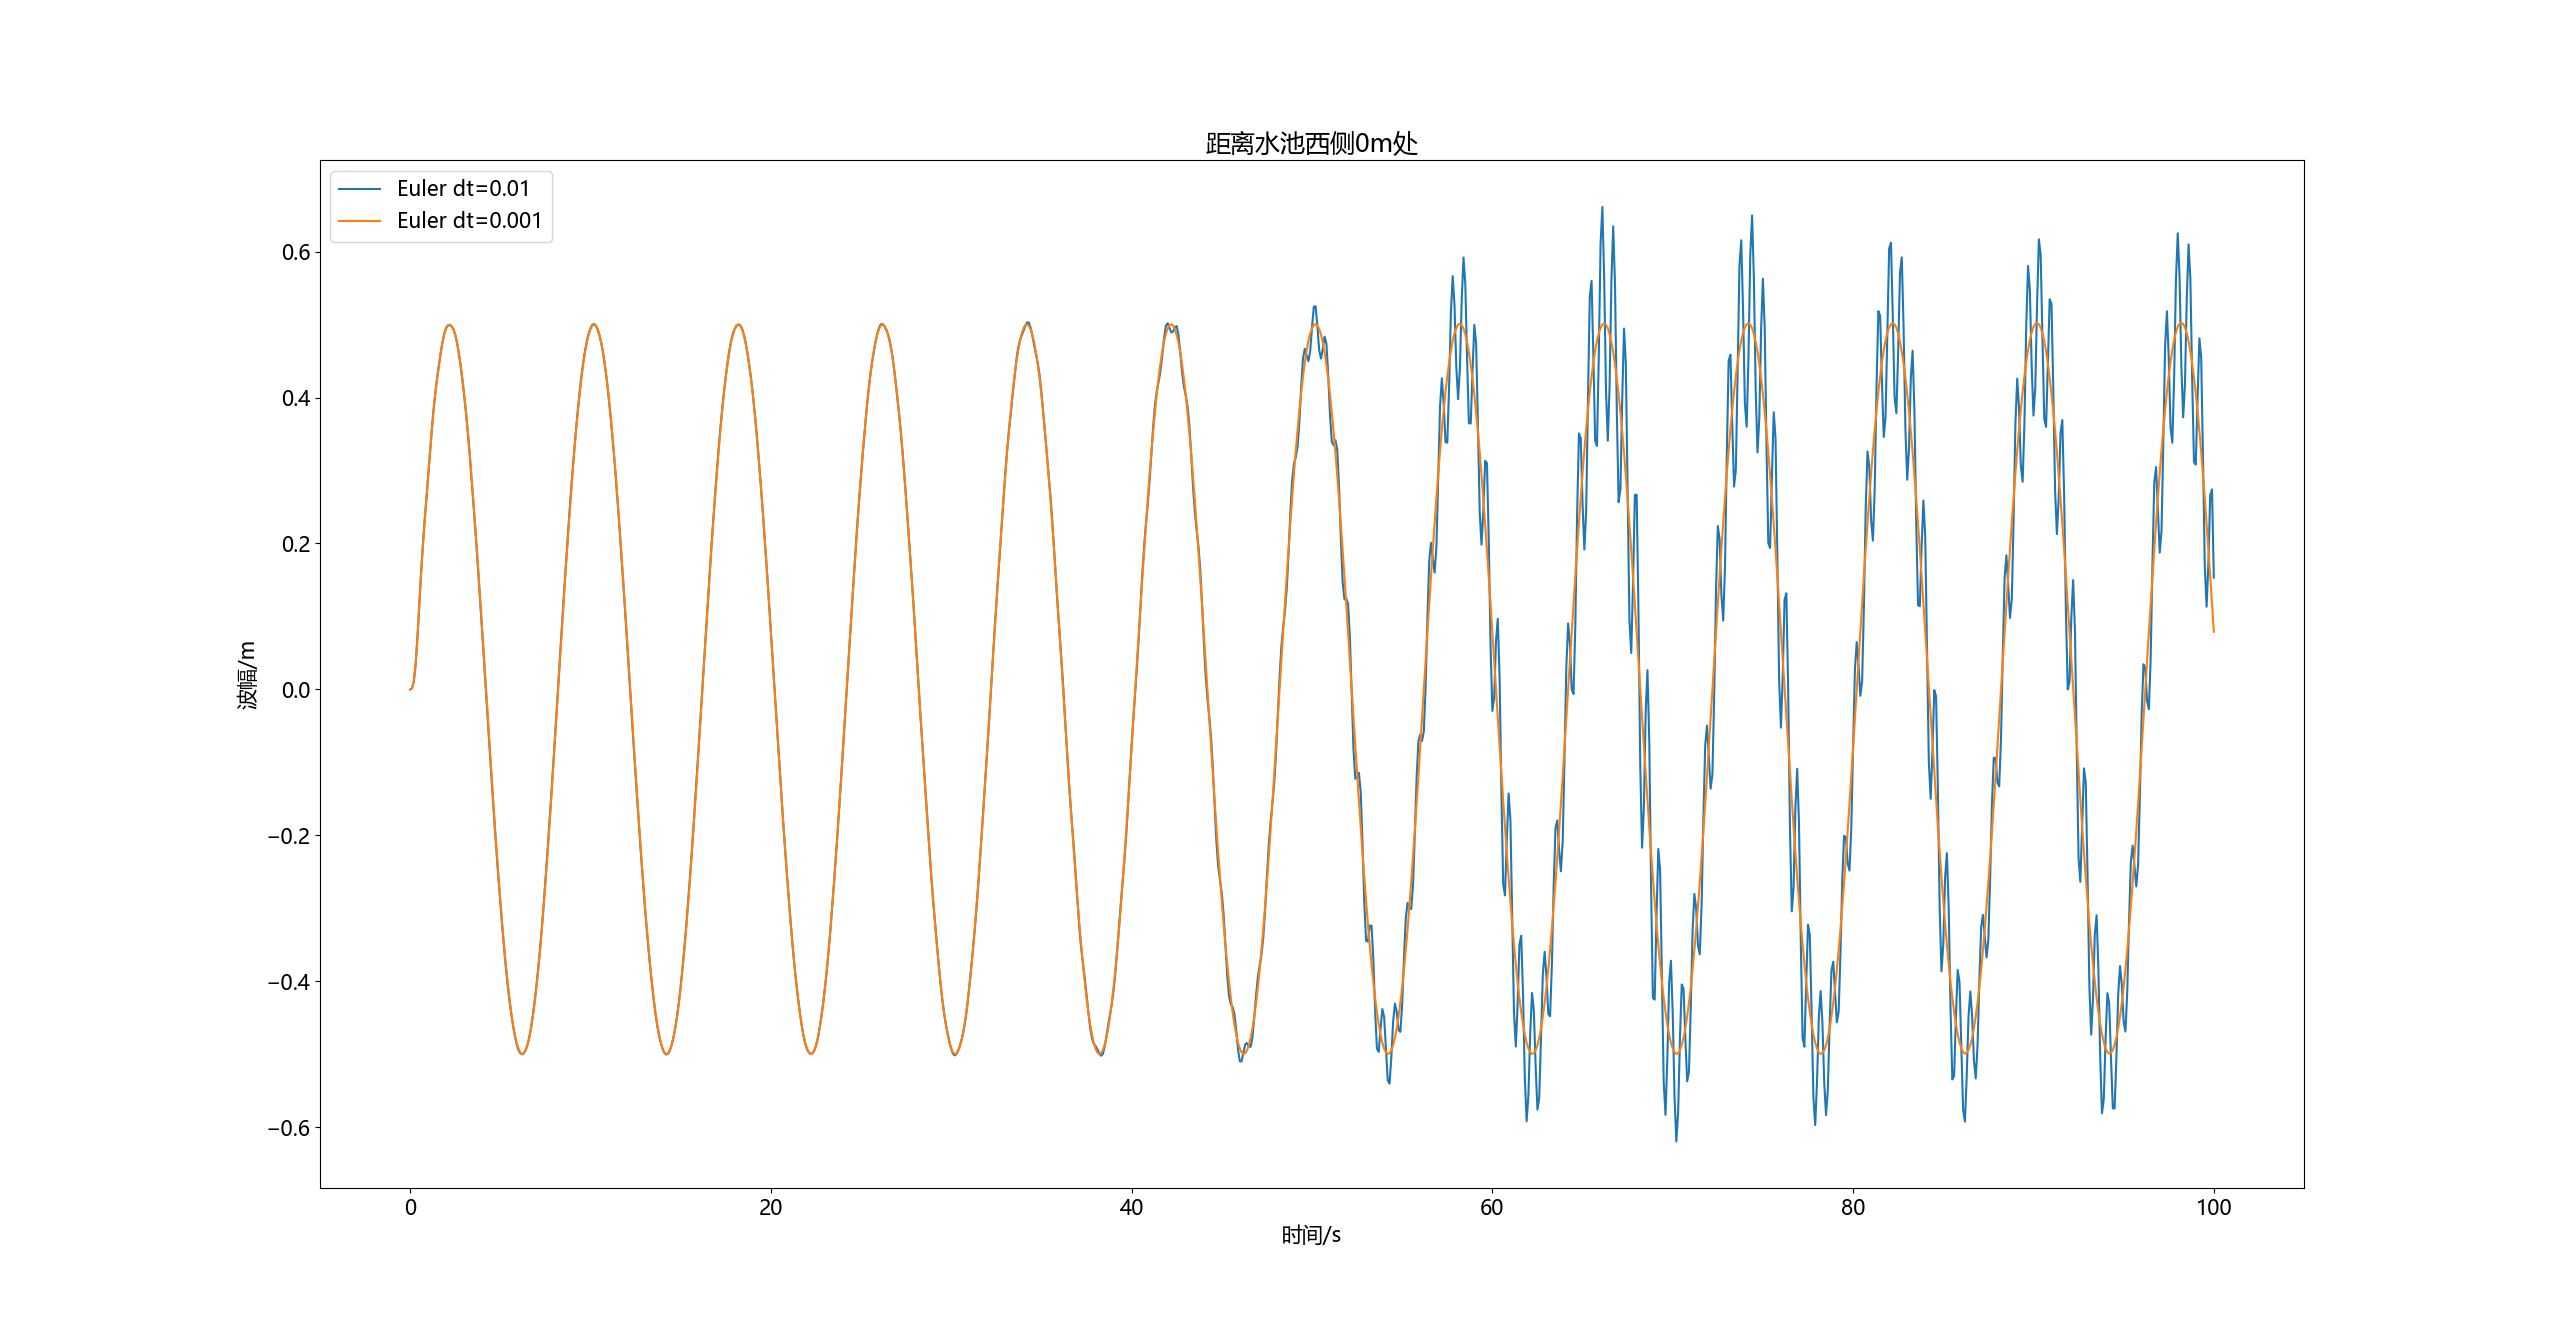
\includegraphics[width=\textwidth]{waveGeneration.png}
\end{figure}

It can be seen that as time increases, the calculation does not converge at $\ Delta t=0.01 \ mbox {s} $, indicating that the CFL condition is only a necessary condition and not sufficient. But when $\ Delta t=0.001 \ mbox {s} $, the amplitude and period are the same as the expected input. Draw the frequency domain graph for $\ Delta t=0.001 \ mbox {s} $ as follows

\begin{figure}[htbp]
	\center{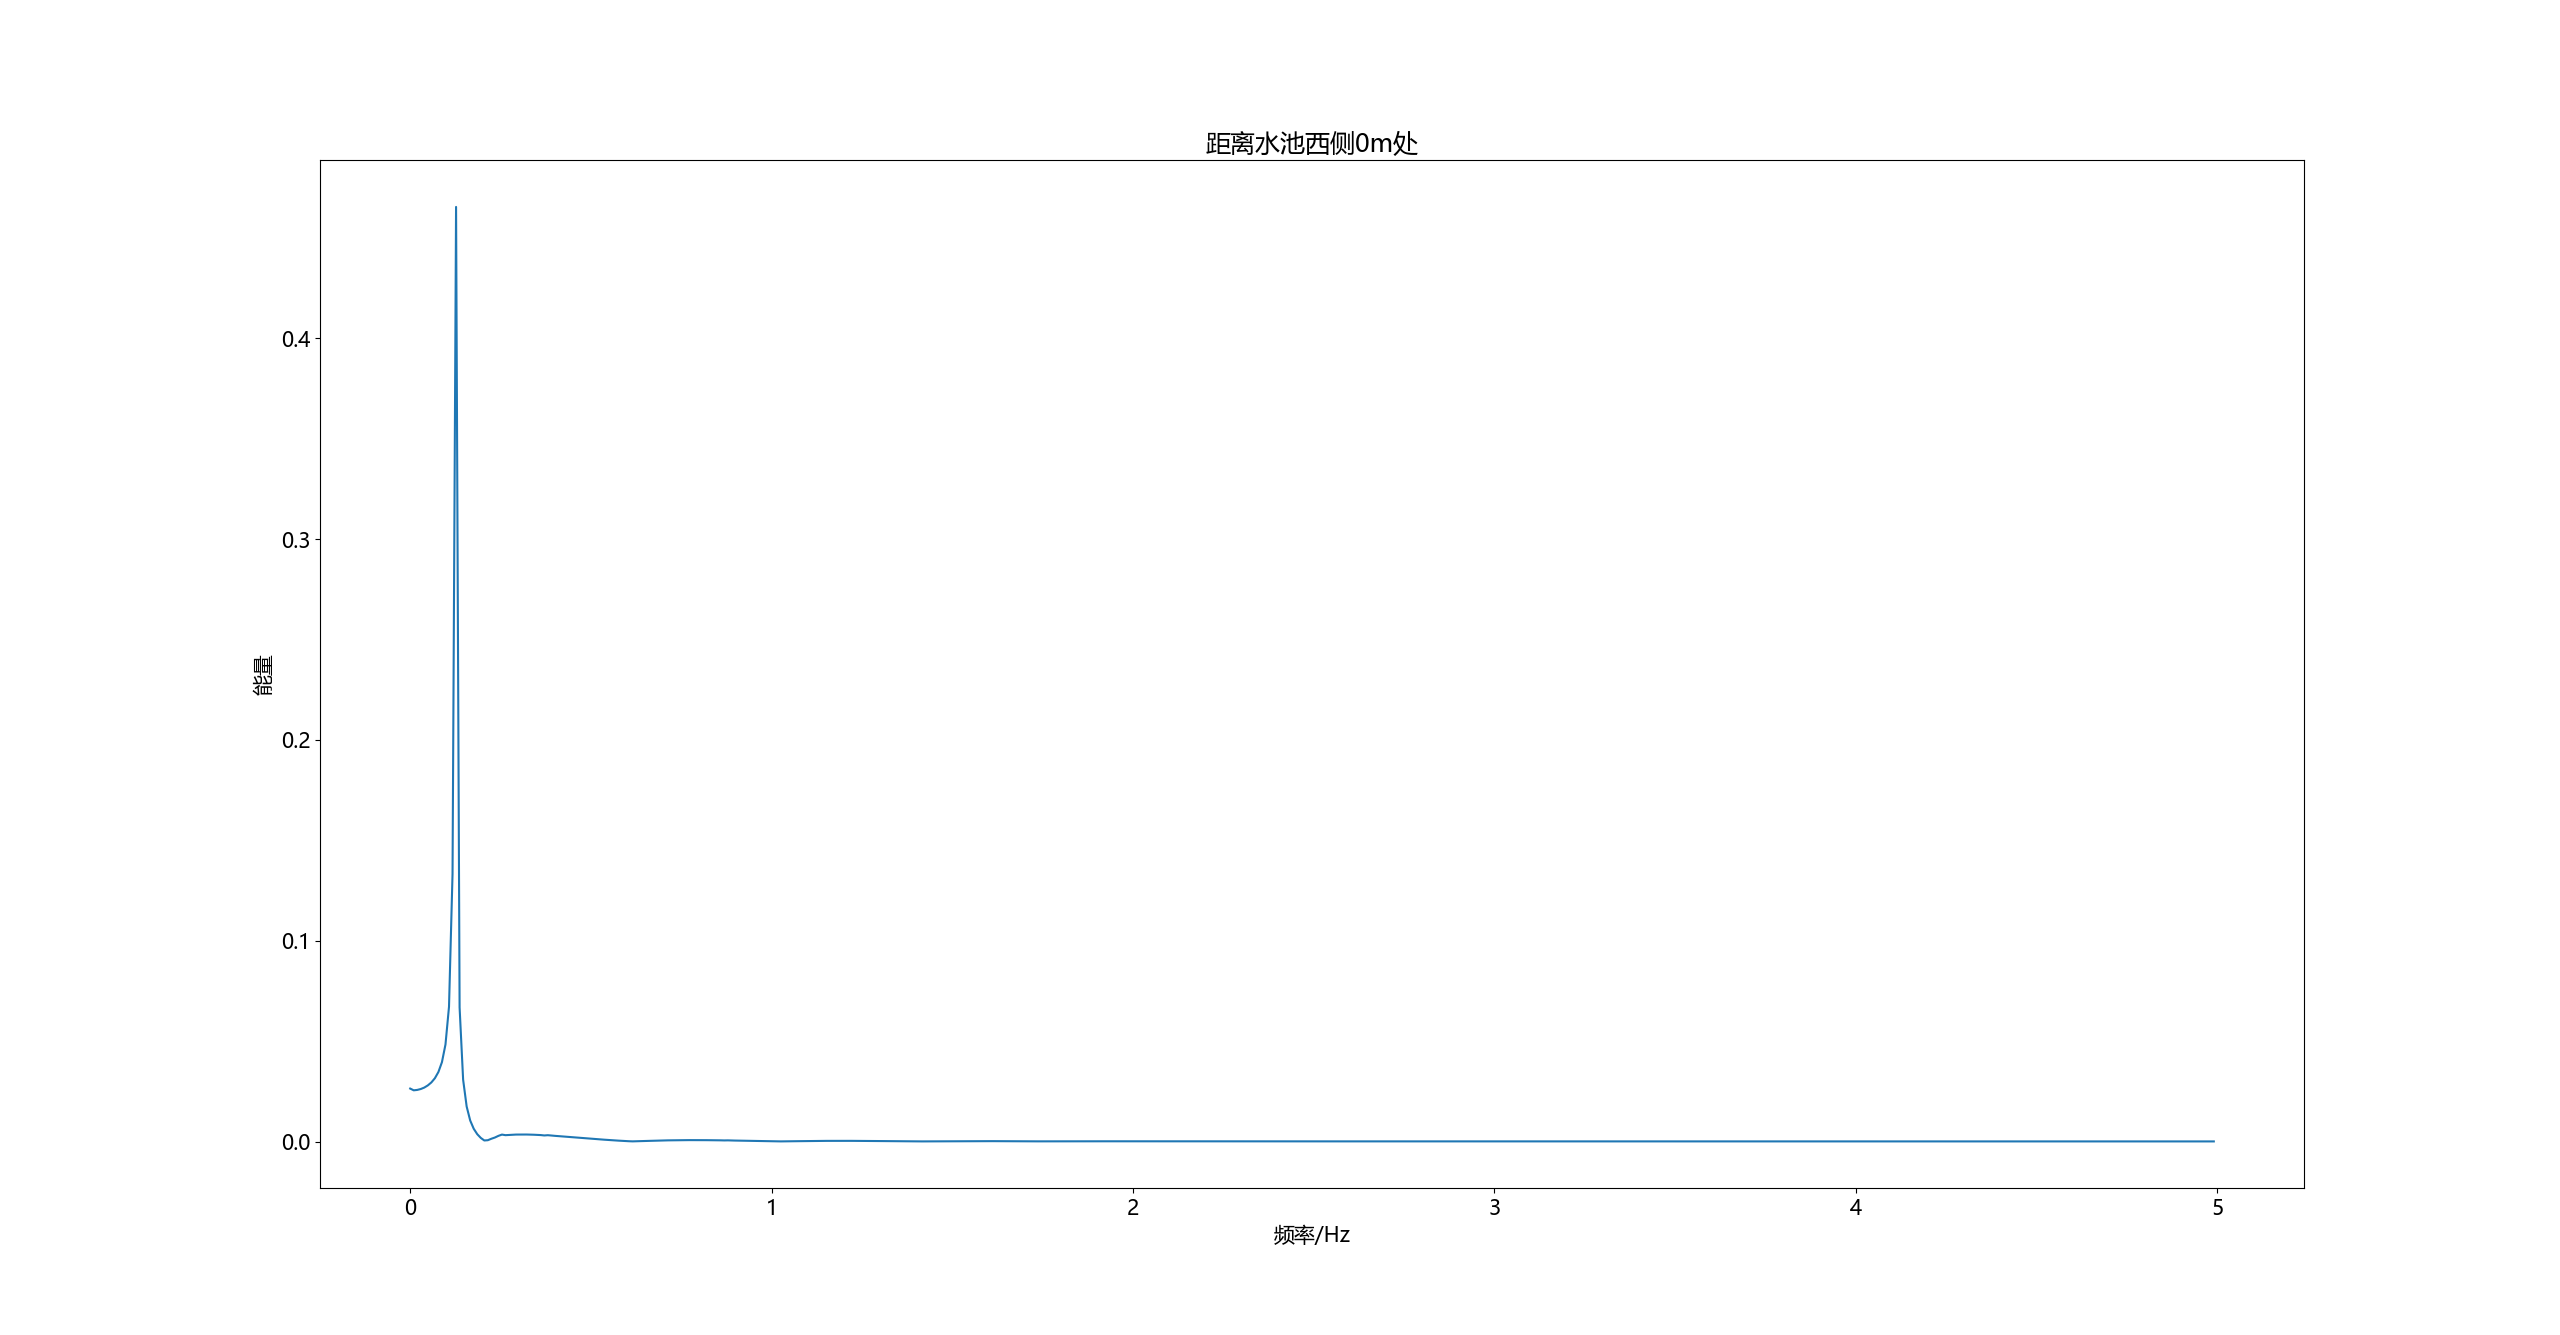
\includegraphics[width=0.83\textwidth]{waveGenerationFre.png}}
\end{figure}

It can be seen that the amplitude is $0.46$ and the corresponding frequency is $0.125\mbox{Hz}$, which is basically consistent with the parameters of the input wave.

\subsection{Convergence analysis of time stepping format}\label{sec2}
Using Euler method, Runge Kutta third-order integral, and Runge Kutta fourth-order integral respectively, with$\Delta t=0.01\mbox{s}$. Observe the time history of the input wave on the west side of the pool and obtain the following figure

\begin{figure}[htbp]
	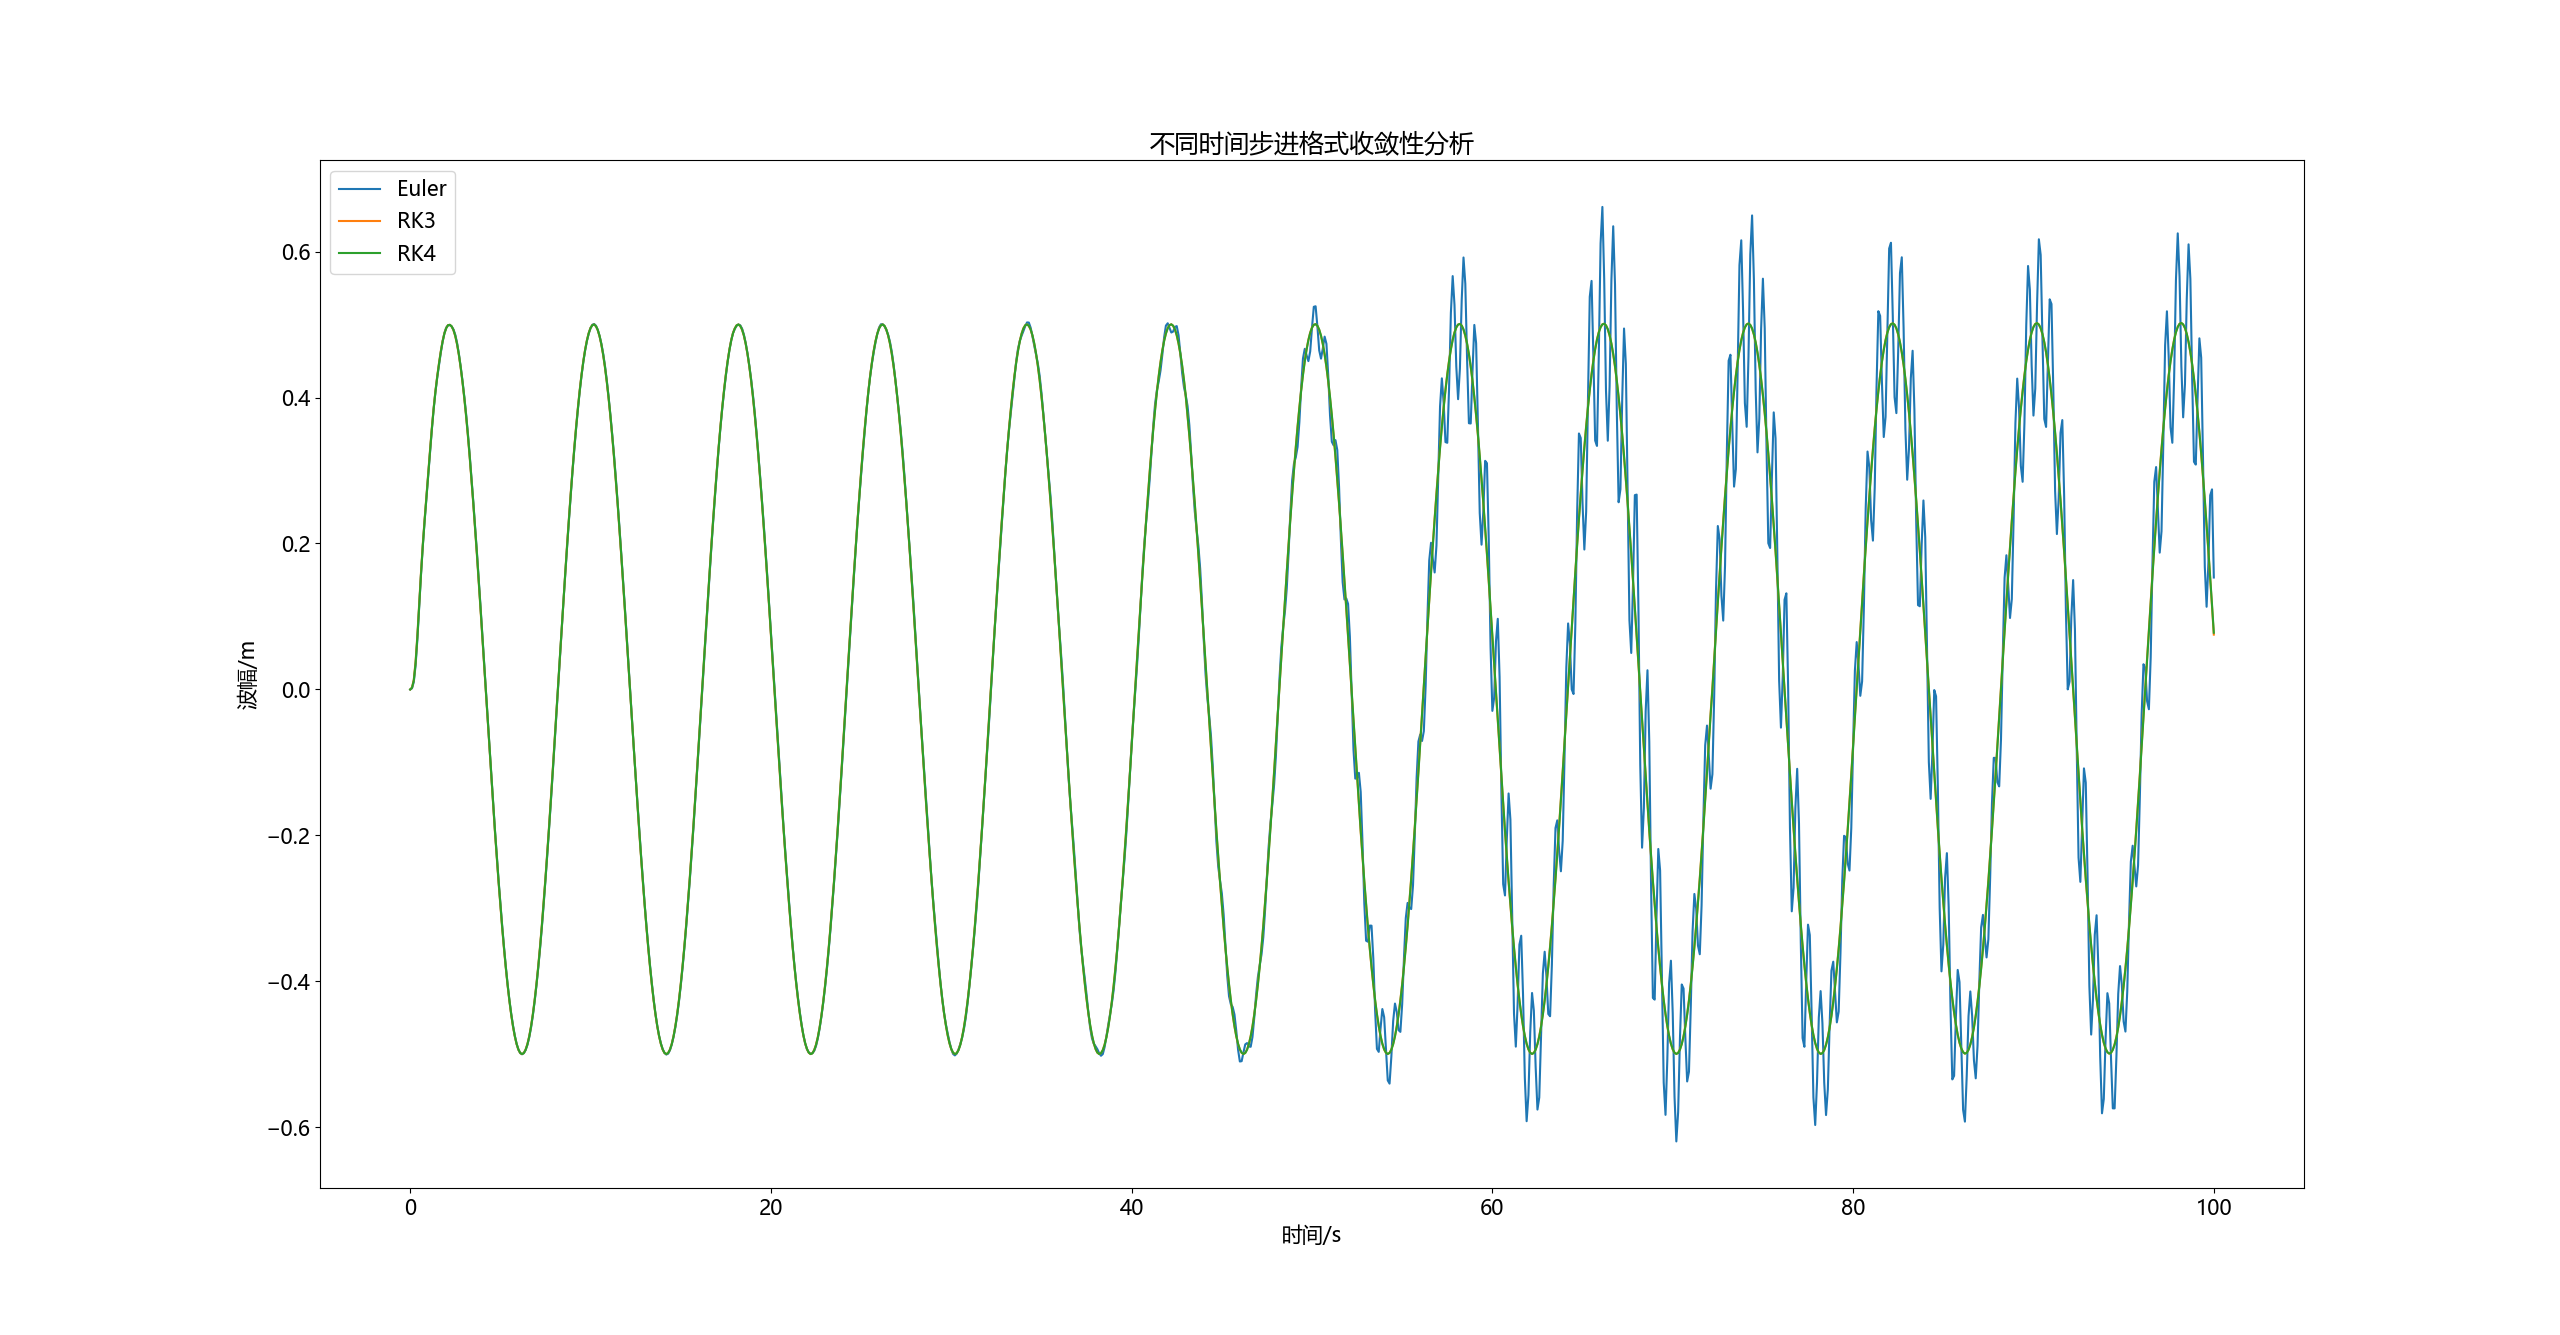
\includegraphics[width=\textwidth]{timeStep.png}
\end{figure}

It can be seen that at the same time step, the results of Runge Kutta third-order and Runge Kutta fourth-order are similar, and their convergence is significantly better than the Euler method.

\subsection{Analysis of numerical dissipation in upwind format}\label{sec3}
Observe the time history of waves in the middle of the pool using the Euler method. Let $\Delta t=0.001\mbox{s}$. Compare the calculation results of different grid sizes in $x$ direction
\begin{figure}[htbp]
	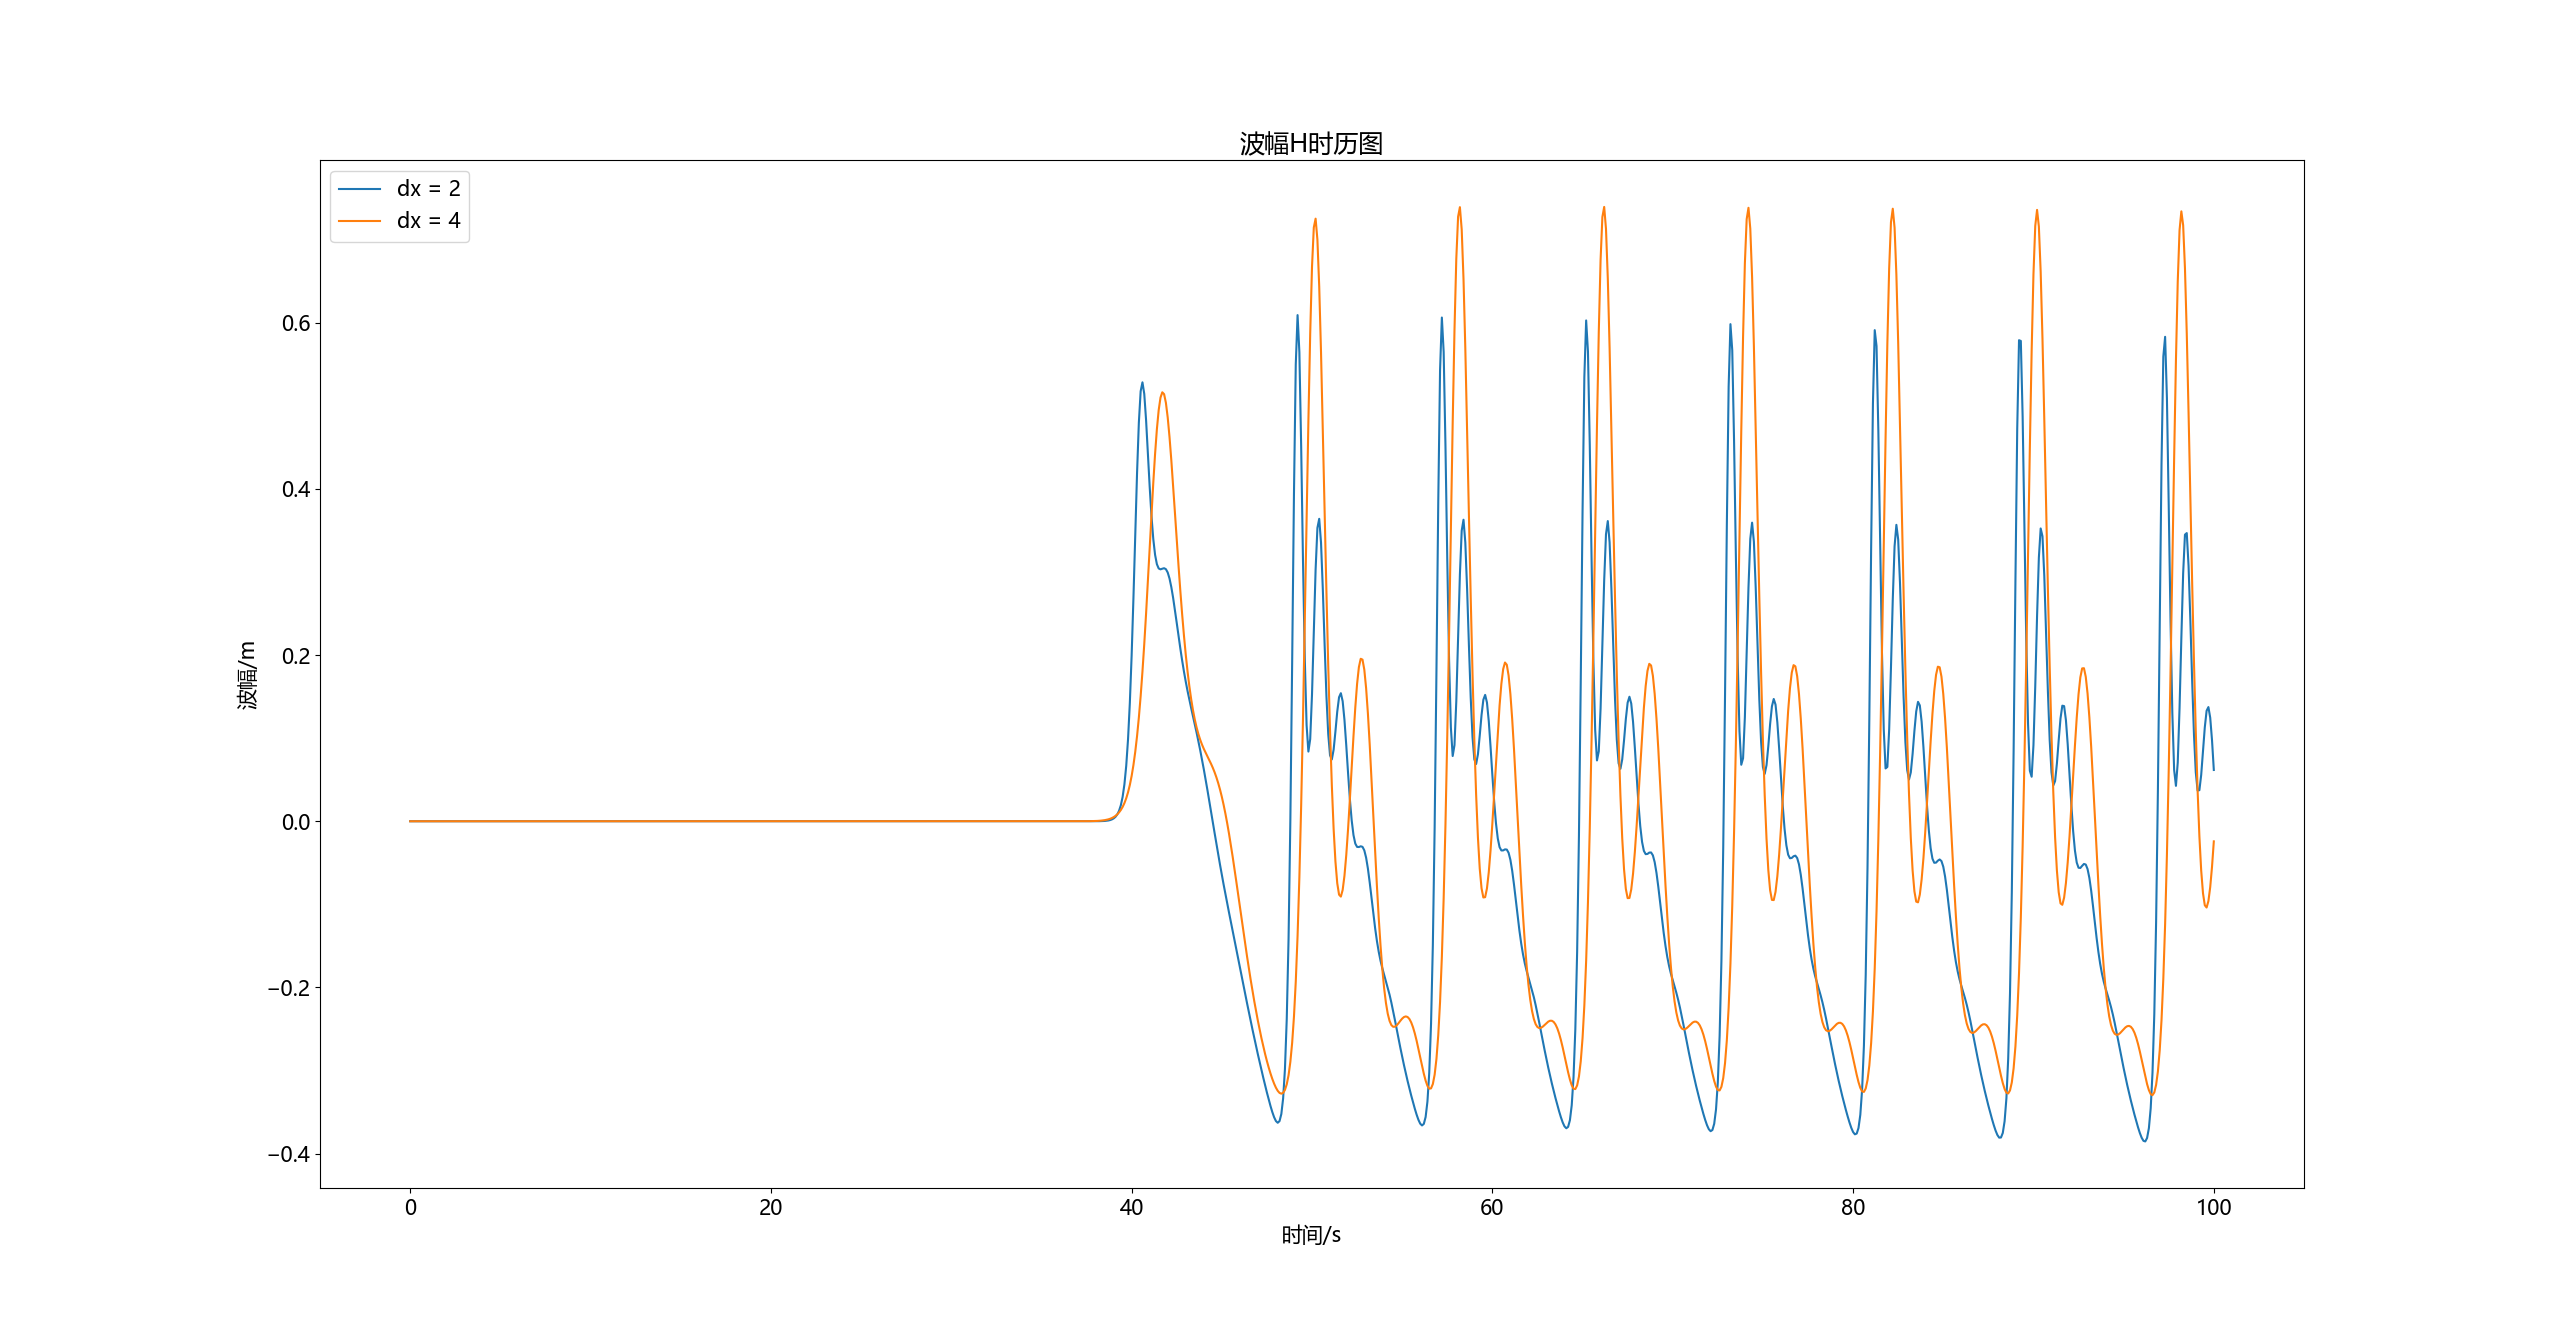
\includegraphics[width=\textwidth]{numericalDispersion.png}
\end{figure}

It is concluded that
\begin{itemize}
	\item As the waves propagate, the wavefront becomes steep and oscillations appear behind the waves.
	\item The larger the grid, the greater the numerical oscillation and the more unstable the calculation results.
	\item The upper and lower bounds of waves changes from $-0.5 - 0.5$ to $-0.38 - 0.62$. It can be seen that the waves are moving upwards as a whole.
	\item The period of waves remains at $8\mbox{s}$.
	\item According to the theory of harmonic waves, calculate the wave propagation speed at a depth of $10\mbox{m}$. First, from dispersion relation
	$$\omega^2 = gk\tanh kh$$
	we get $k = 0.1033\mbox{m}^{-1}$, then calculate wave speed $c = 7.6\mbox{m/s}$. Therefore, according to the theory of harmonic waves, waves should arrive at the center of the tank at $$t = 400/7.6=52.6\mbox{s}$$. But the actual time is $40\mbox{s}$. This reflects that the gradually rising changes in the seabed have accelerated the propagation speed of waves.
\end{itemize}

\subsection{The variation of wave parameters on terrain}\label{sec4}
Observe when $t=50\mbox{s}$, the wave pattern is
\begin{figure}[htb]
	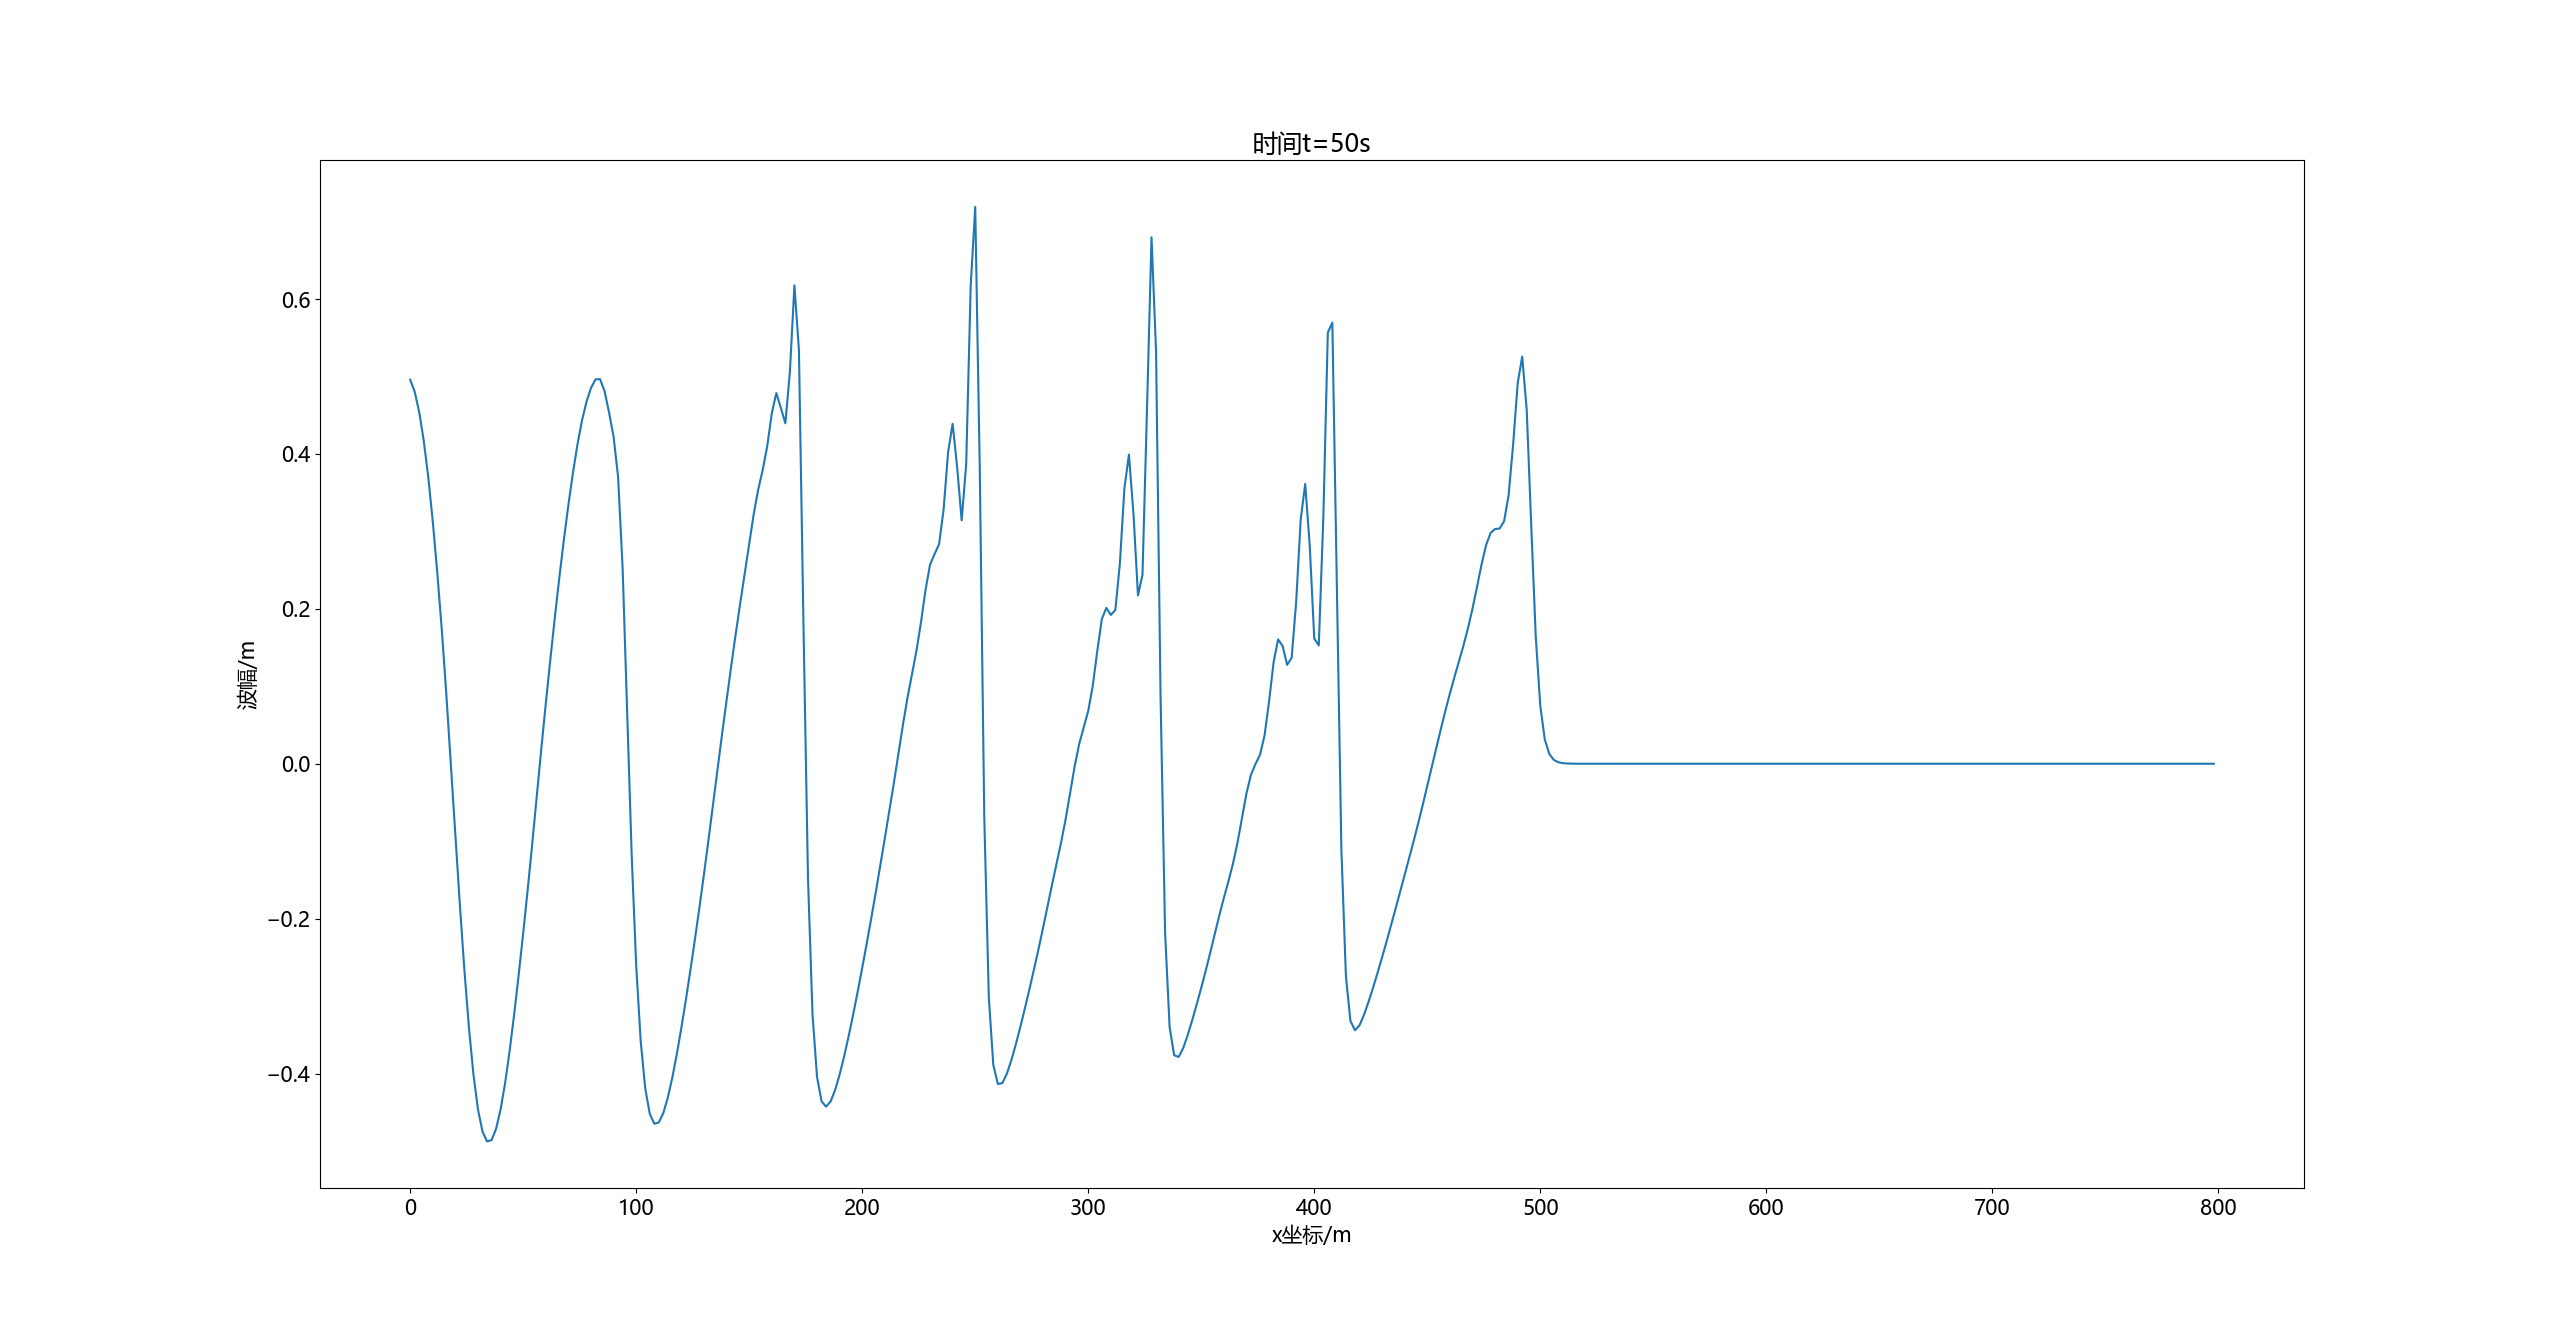
\includegraphics[width=\textwidth]{waveShape.png}
\end{figure}

Combining \ref{sec3}, we get
\begin{itemize}
	\item As the waves propagate, the wavefront becomes steeper, oscillations appear behind the waves, and the waves move upward as a whole.
	\item Wave length increases gradually/ From $73\mbox{m}$ on the weat boundary, to $80\mbox{m}$ at the center of the tank, According to harmonic wave theory, when water depth is $10\mbox{m}$, wave length should be
	$$\lambda = \frac{2\pi}{0.1033}\mbox{m} = 60.82\mbox{m}$$
	This reflects the gradually rising seabed changes that followed, the wavelength of the waves increased.
\end{itemize}

\subsection{Comparison of Calculation Time}
In order to compare the calculation time of different time step formats and time intervals, the numerical experiment table is recorded as follows
\center{
\begin{tabular}{|c|c|c|c|}
	\hline
	& Euler Method & RK-3 & RK-4 \\
	\hline
	$\Delta t=0.01\mbox{s}$ & 9.07\mbox{s} &  11.43\mbox{s}& 16.52\mbox{s}\\
	\hline
	$\Delta t=0.001\mbox{s}$ & 30.34\mbox{s} & 52.34\mbox{s} &  99.60\mbox{s}\\
\end{tabular}}

\newpage
Combining \ref{sec2}, it can be seen that in this example, the Runge Kutta third-order or Runge Kutta fourth-order method can balance computational efficiency and accuracy when $\Delta t=0.01\mbox{s}$.

\subsection{Observation of Water Quality Point Velocity}

In the calculation, velocity in $y$ direction is less than $2\times10^{-4}\mbox{m/s}$ which reflects that the influence of Coriolis force is minimal.

Draw the time history of velocity in $x$ on the west side of the pool and in the middle of the pool as follows
\begin{figure}[htbp]
	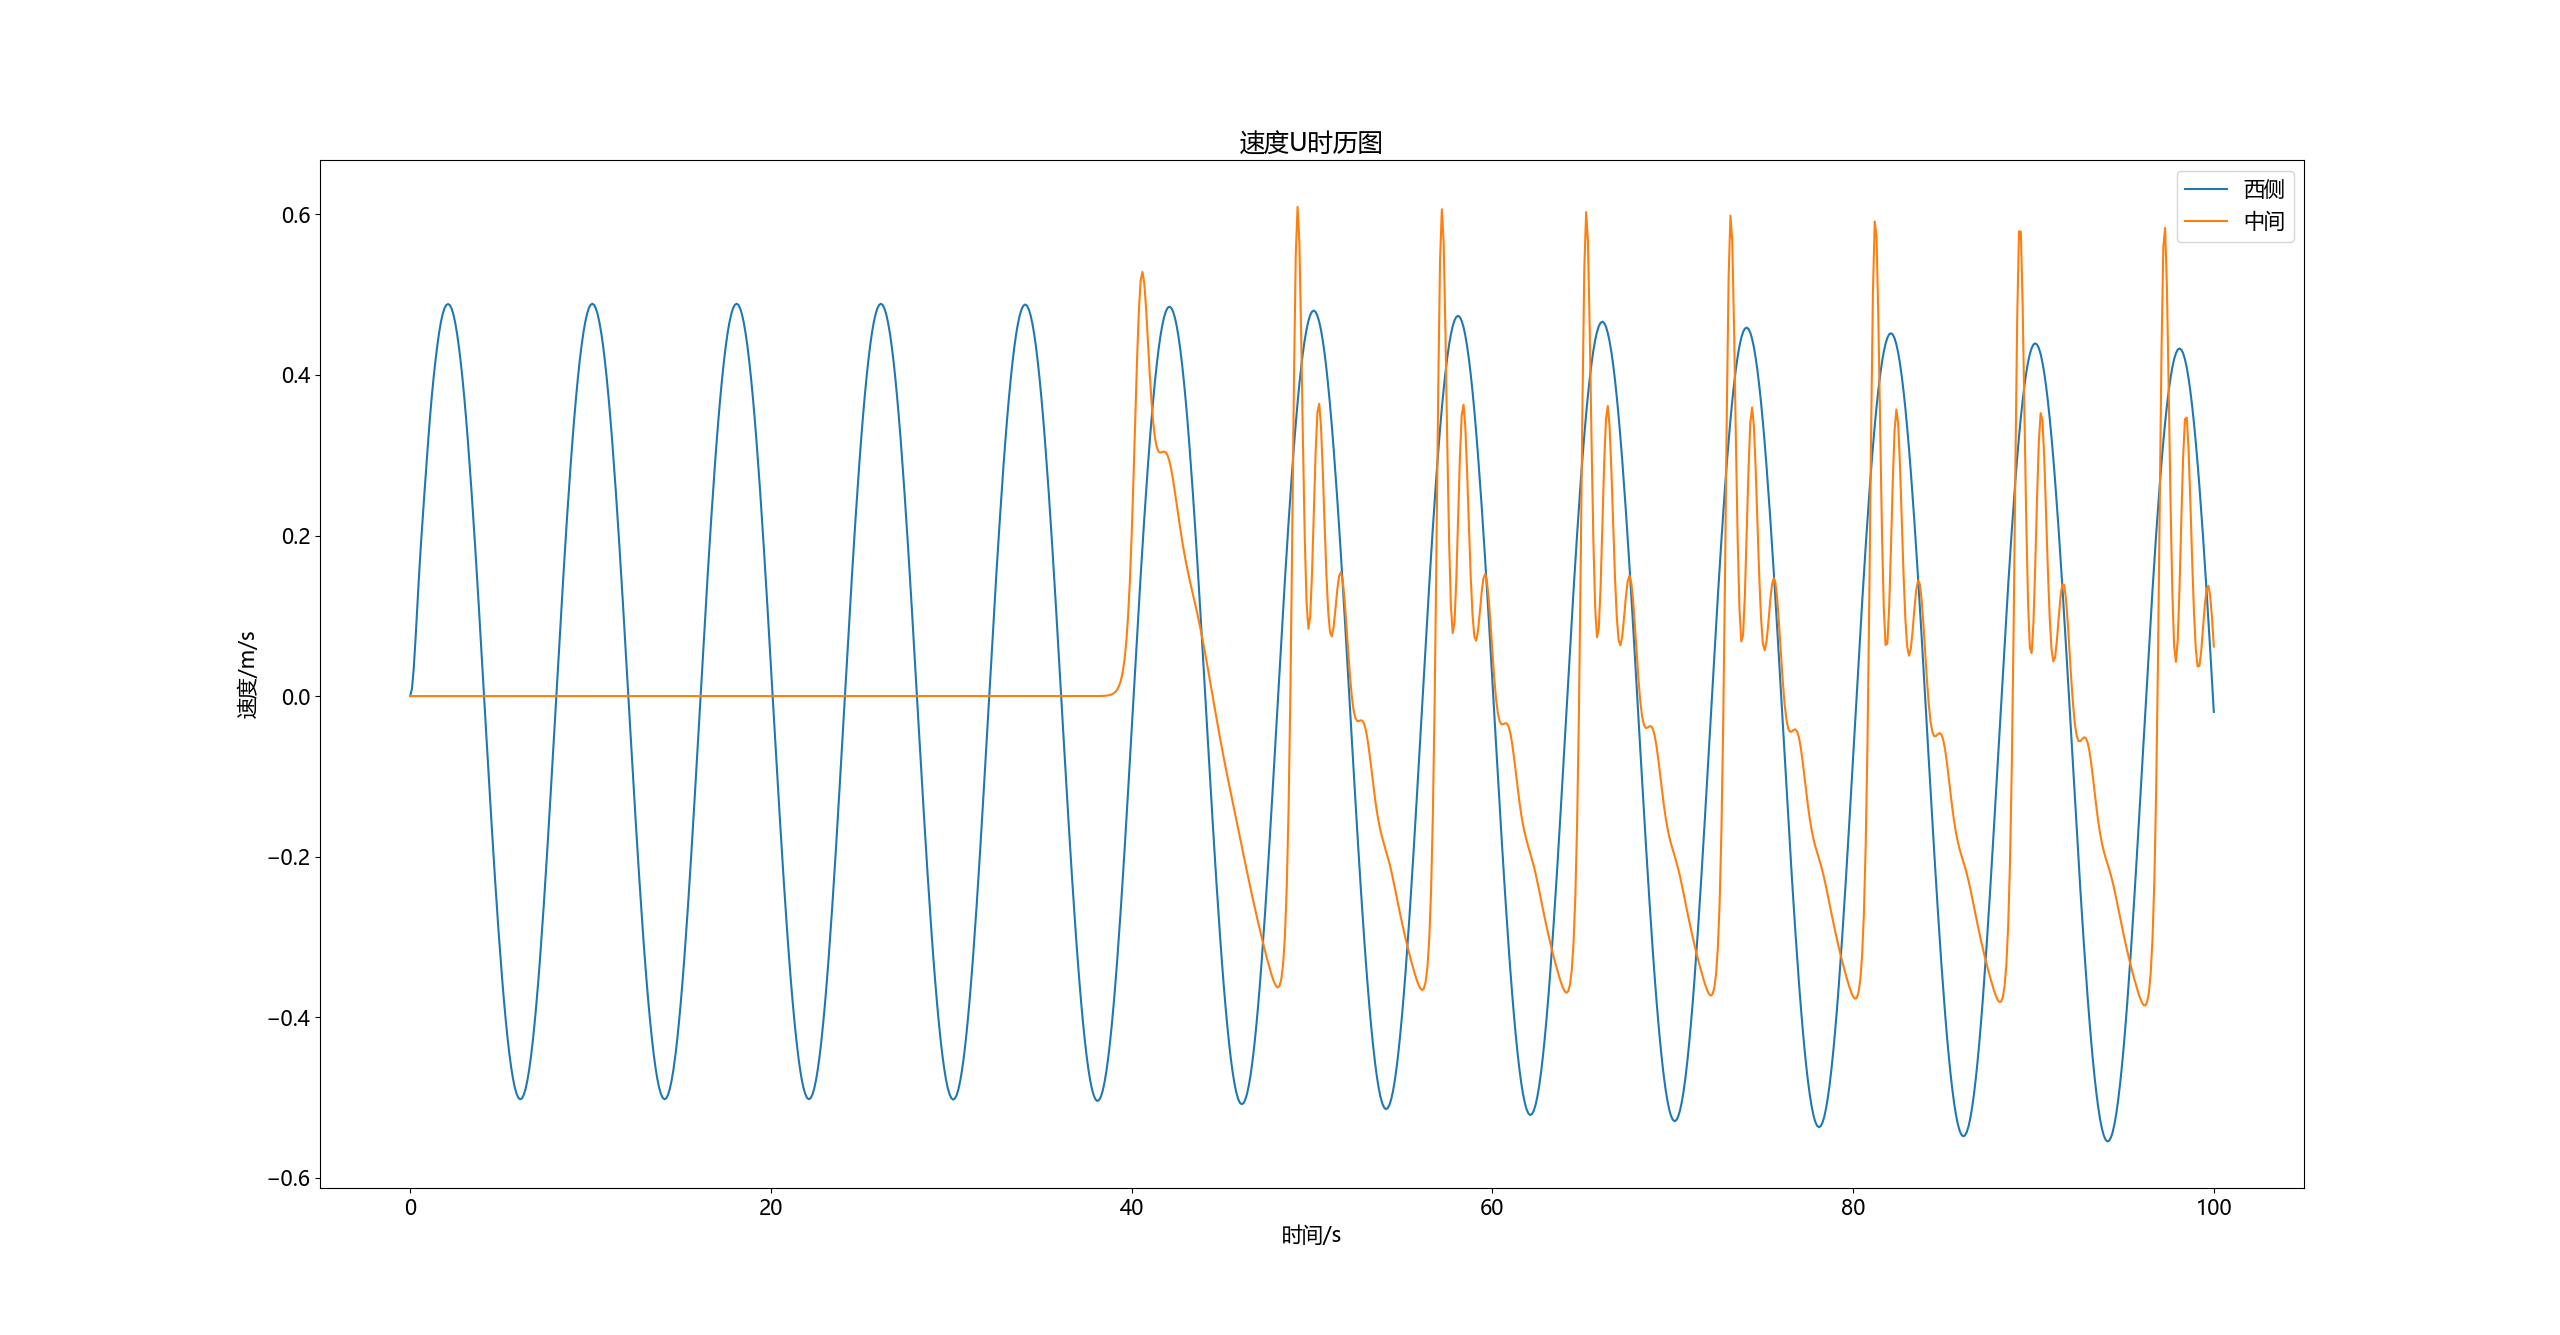
\includegraphics[width=\textwidth]{velocity.png}
\end{figure}

It can be seen that the trend and magnitude of the horizontal velocity $U $are similar to the amplitude $H $, which is also consistent with the input:
\begin{equation}
	U = A\sqrt{\frac{g}{D}} \approx A
\end{equation}

\newpage
\section{Conclusion}

\begin{enumerate}
	\item The calculated shape of the wave shows that the wavefront becomes steep and the background becomes gentle, which is consistent with actual observations.\upcite{5}
	\item The wave amplitude in this calculation is relatively accurate, but in reality, as the water depth becomes shallower, the wave amplitude on the water surface will increase.
	\item In this calculation, the frequency of the waves did not change and the wavelength became longer, which is inconsistent with the facts. In reality, as the water depth becomes shallower, the period should increase and the wavelength should decrease.
	\item Combining \ref{sec3} and \ref{sec4} and formula
	$$c = \frac{\lambda}{T}$$
	it can be seen that the increase in wave velocity in this wave simulation is due to the increase in wavelength.
\end{enumerate}

%\section{参考文献}

\newpage
\begin{thebibliography}{1}
	\bibitem{1} Yingzhong Liu. Computational Ship Fluid Dynamics[M]. 54-56.
	\bibitem{2} J. J. Dronkers, Tidal Computations in Rivers and Coastal Waters, John Wiley \& Sons, Inc., New York (1964).
	\bibitem{3} Charles L. Mader. Numerical Modelling of Water Waves, CRC Press, Boca Raton (2004). 31-42.
	\bibitem{4} Fengyan Shi, et al. A high-order adaptive time-stepping TVD solver for Boussinesq modeling of breaking waves and coastal inundation, Ocean Modelling, Volumes 43–44, 2012, Pages 36-51.
	\bibitem{5} Yifei Zeng. Marine Engineering Environment[M]. Shanghai: Shanghai Jiao Tong University Press (2007).
\end{thebibliography}
\end{document}